\documentclass{beamer}
\usepackage{tikz,amsmath,hyperref,graphicx,stackrel,animate,tipa}
\usetikzlibrary{positioning,shadows,arrows,shapes,calc}
\newcommand{\ipa}[1]{\textipa{#1}}
\newcommand{\argmax}{\operatornamewithlimits{argmax}}
\newcommand{\argmin}{\operatornamewithlimits{argmin}}
\newcommand{\dbar}[1]{\overline{\overline{#1}}}
\mode<presentation>{\usetheme{Frankfurt}}
\DeclareMathOperator*{\softmax}{softmax}
\AtBeginSection[]
{
  \begin{frame}<beamer>
    \frametitle{Outline}
    \tableofcontents[currentsection,currentsubsection]
  \end{frame}
}
\title{Baum-Welch and Viterbi}
\author{Mark Hasegawa-Johnson\\These slides are in the public domain}
\date{ECE 417: Multimedia Signal Processing}  
\begin{document}

% Title
\begin{frame}
  \maketitle
\end{frame}

% Title
\begin{frame}
  \tableofcontents
\end{frame}

%%%%%%%%%%%%%%%%%%%%%%%%%%%%%%%%%%%%%%%%%%%%
\section[Review]{Review: Hidden Markov Models}
\setcounter{subsection}{1}


\begin{frame}
  \frametitle{Hidden Markov Model}

  \begin{center}
    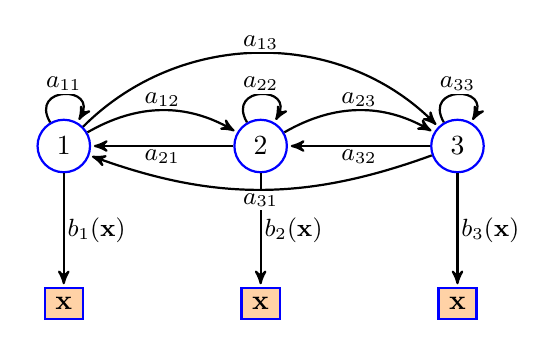
\begin{tikzpicture}[->,>=stealth',shorten >=1pt,auto,node distance=3cm,thick,
        state/.style={circle,thick,draw=blue,text=black,text centered,text width=0.25cm},
        obs/.style={rectangle,thick,draw=blue,text=black,fill=orange!35!white,text centered,text width=0.25cm}
      ]
      \node[state] (q1) at (0,0) {1};
      \node[state] (q2) at (2.5,0) {2};
      \node[state] (q3) at (5,0) {3};
      \node[obs] (x1) at (0,-2) {$\mathbf{x}$};
      \node[obs] (x2) at (2.5,-2) {$\mathbf{x}$};
      \node[obs] (x3) at (5,-2) {$\mathbf{x}$};
      \path[every node/.style={font=\sffamily\small,
  	  fill=white,inner sep=1pt}]
      (q1) edge [out=120,in=60,looseness=4] node {$a_{11}$} (q1)
      edge [out=30,in=150] node {$a_{12}$} (q2)
      edge [out=45,in=135] node {$a_{13}$} (q3)
      edge [out=-90,in=90] node {$b_1(\mathbf{x})$} (x1)
      (q2) edge [out=120,in=60,looseness=4] node {$a_{22}$} (q2)
      edge [out=180,in=0] node {$a_{21}$} (q1)
      edge [out=30,in=150] node {$a_{23}$} (q3)
      edge [out=-90,in=90] node {$b_2(\mathbf{x})$} (x2)
      (q3) edge [out=120,in=60,looseness=4] node {$a_{33}$} (q3)
      edge [out=180,in=0] node {$a_{32}$} (q2)
      edge [out=-160,in=-20] node {$a_{31}$} (q1)
      edge [out=-90,in=90] node {$b_3(\mathbf{x})$} (x3);
    \end{tikzpicture}
  \end{center}
  \begin{enumerate}
  \item Start in state $q_t=i$ with pmf $\pi_i$.
  \item Generate an observation, $\mathbf{x}$, with pdf $b_i(\mathbf{x})$.
  \item Transition to a new state, $q_{t+1}=j$, according to pmf $a_{ij}$.
  \item Repeat.
  \end{enumerate}
\end{frame}


\begin{frame}
  \frametitle{The Three Problems for an HMM}

  \begin{enumerate}
  \item {\bf Recognition:} Given two different HMMs, $\Lambda_1$ and
    $\Lambda_2$, and an observation sequence $X$.  Which HMM was more
    likely to have produced $X$?  In other words, 
    $p(X|\Lambda_1)>p(X|\Lambda_2)$?
  \item {\bf Segmentation:} What is $p(q_t=i|X,\Lambda)$?
  \item {\bf Training:} Given an initial HMM $\Lambda$, and an
    observation sequence $X$, can we find $\Lambda'$ such that
    $p(X|\Lambda') > p(X|\Lambda)$?
  \end{enumerate}
\end{frame}

\begin{frame}
  \frametitle{The Forward Algorithm}

  Definition:
  $\alpha_t(i)\equiv\Pr\left\{\mathbf{x}_1,\ldots,\mathbf{x}_t,q_t=i|\Lambda\right\}$.
  Computation:
  \begin{enumerate}
  \item {\bf Initialize:}
    \[
    \alpha_1(i) = \pi_i b_i(\mathbf{x}_1),~~~1\le i\le N
    \]
  \item {\bf Iterate:}
    \begin{align*}
      \alpha_{t}(j) &= \sum_{i=1}^N \alpha_{t-1}(i) a_{i,j}b_j(\mathbf{x}_t),~~1\le j\le N,~2\le t\le T
    \end{align*}
  \item {\bf Terminate:}
    \[
    \Pr\left\{\mathbf{X}|\Lambda\right\} = \sum_{i=1}^N \alpha_T(i)
    \]
  \end{enumerate}
\end{frame}
  
\begin{frame}
  \frametitle{The Backward Algorithm}

  Definition: $\beta_t(i) \equiv
  \Pr\left\{\mathbf{x}_{t+1},\ldots,\mathbf{x}_T|q_t=i,\Lambda\right\}$.
  Computation:
  \begin{enumerate}
  \item {\bf Initialize:}
    \[
    \beta_T(i) = 1,~~~1\le i\le N
    \]
  \item {\bf Iterate:}
    \begin{align*}
      \beta_{t}(i) &= \sum_{j=1}^N a_{i,j}b_j(\mathbf{x}_{t+1})\beta_{t+1}(j),~~1\le i\le N,~1\le t\le T-1
    \end{align*}
  \item {\bf Terminate:}
    \[
    \Pr\left\{\mathbf{X}|\Lambda\right\} = \sum_{i=1}^N \pi_ib_i(\mathbf{x}_1)\beta_1(i)
    \]
  \end{enumerate}
\end{frame}

\begin{frame}
  \frametitle{Segmentation}

  \begin{enumerate}
  \item {\bf The State Posterior:}
    \begin{align*}
      \gamma_t(i) & = \Pr\left\{q_t=i|\mathbf{X},\Lambda\right\}
      = \frac{\alpha_t(i)\beta_t(i)}{\sum_{k=1}^N\alpha_t(k)\beta_t(k)}
    \end{align*}
  \item {\bf The Segment Posterior:}
    \begin{align*}
      \xi_t(i,j) & = \Pr\left\{q_t=i,q_{t+1}=j|\mathbf{X},\Lambda\right\}\\
      &= \frac{\alpha_t(i)a_{i,j}b_j(\mathbf{x}_{t+1})\beta_{t+1}(j)}{\sum_{k=1}^N\sum_{\ell=1}^N\alpha_t(k)a_{k\ell}b_\ell(\mathbf{x}_{t+1})\beta_{t+1}(\ell)}
    \end{align*}
  \end{enumerate}
\end{frame}


\begin{frame}
  \frametitle{The Three Problems for an HMM}

  \begin{enumerate}
  \item {\bf Recognition:} Given two different HMMs, $\Lambda_1$ and
    $\Lambda_2$, and an observation sequence $X$.  Which HMM was more
    likely to have produced $\mathbf{X}$?  In other words, 
    $\Pr\left\{\mathbf{X}|\Lambda_1)>p(\mathbf{X}|\Lambda_2\right\}$?
  \item {\bf Segmentation:} What is $\Pr\left\{q_t=i|\mathbf{X},\Lambda\right\}$?
  \item {\bf Training:} Given an initial HMM $\Lambda$, and an
    observation sequence $\mathbf{X}$, can we find $\Lambda'$ such that
    $\Pr\left\{\mathbf{X}|\Lambda'\right\} > \Pr\left\{\mathbf{X}|\Lambda\right\}$?
  \end{enumerate}
\end{frame}


%%%%%%%%%%%%%%%%%%%%%%%%%%%%%%%%%%%%%%%%%%%%
\section[ML]{Training: Maximum-Likelihood with a Given State Sequence}
\setcounter{subsection}{1}

\begin{frame}
  \frametitle{Maximum Likelihood Training}
  
  Suppose we're given several observation sequences of the form
  $\mathbf{X}=[\mathbf{x}_1,\ldots,\mathbf{x}_T]$.  Suppose, also, that we have some
  initial guess about the values of the model parameters (our initial
  guess doesn't have to be very good).  Maximum likelihood training
  means we want to compute a new set of parameters,
  $\Lambda'=\left\{\pi_i',a_{i,j}',b_j'(\mathbf{x})\right\}$ that maximize
  $\Pr\left\{\mathbf{X}|\Lambda'\right\}$.
  \begin{enumerate}
  \item {\bf Initial State Probabilities:} Find values of $\pi_i'$, $1\le
    i\le N$, that maximize $\Pr\{X|\Lambda'\}$.
  \item {\bf Transition Probabilities:} Find values of $a_{i,j}'$, $1\le
    i,j\le N$, that maximize $\Pr\{X|\Lambda'\}$.
  \item {\bf Observation Probabilities:} Learn $b_j'(\mathbf{x})$.  What does that
    mean, actually?
  \end{enumerate}
\end{frame}

\begin{frame}
  \frametitle{Learning the Observation Probabilities}

  There are three common ways of representing the observation probabilities, $b_j(\mathbf{x})$.
    \begin{enumerate}
    \item Vector quantize $\mathbf{x}$, using some VQ method.  Suppose
      $\mathbf{x}$ is the $k^{\textrm{th}}$ codevector; then we just need
      to learn $b_j(k)$ such that
      \[
      b_j(k)\ge 0,~~~\sum_{k=0}^{K-1} b_j(k)=1
      \]
    \item Model $b_j(k)$ as a Gaussian, or some other parametric pdf
      model, and learn its parameters.
    \item Model $b_j(k)$ as a neural net, and learn its parameters.
    \end{enumerate}
\end{frame}
  
\begin{frame}
  \frametitle{Maximum Likelihood Training}
  
  For now, suppose that we have the following parameters that we need to learn:
  \begin{enumerate}
  \item {\bf Initial State Probabilities:} $\pi_i'$ such that
    \[
    \pi_i' \ge 0,~~~\sum_{i=1}^N \pi_i' = 1
    \]
  \item {\bf Transition Probabilities:} $a_{i,j}'$ such that
    \[
    a_{i,j}'\ge 0,~~~\sum_{j=1}^N a_{i,j}' =1
    \]
  \item {\bf Observation Probabilities:} $b_j'(k)$ such that
    \[
    b_j'(k)\ge 0,~~~\sum_{k=1}^{K} b_j'(k)=1
    \]
  \end{enumerate}
\end{frame}

\begin{frame}
  \frametitle{Maximum Likelihood Training with Known State Sequence}

  {\bf Impossible assumption}: Suppose that we actually know the state
  sequences, $\mathbf{q}=[q_1,\ldots,q_T]^T$, matching with each
  observation sequence $\mathbf{X}=[\mathbf{x}_1,\ldots,\mathbf{x}_T]$.  Then
  what would be the maximum-likelihood parameters?

\end{frame}

\begin{frame}
  \frametitle{Maximum Likelihood Training with Known State Sequence}

  Our goal is to find $\Lambda=\left\{\pi_i,a_{i,j},b_j(k)\right\}$ in
  order to maximize

  \begin{align*}
    {\mathcal L}(\Lambda) &= \sum_{\text{sequences}}\ln \Pr\{\mathbf{q},\mathbf{X}|\Lambda\}\\
    &= \ln \pi_{q_1} + \ln b_{q_1}(x_1) + \ln a_{q_1,q_2} + b_{q_2}(x_2) + \ldots\\
    &= \sum_{i=1}^N\left(s_i\ln\pi_{i}+\sum_{j=1}^N n_{i,j}\ln a_{i,j} + \sum_{k=1}^Km_{i,k}\ln b_i(k)\right)
  \end{align*}
  where
  \begin{itemize}
  \item $s_i$ is the number of sequences that started with state $i$,
  \item $n_{i,j}$ is the number of frames in which $(q_{t}=i,q_{t+1}=j)$,
  \item $m_{i,k}$ is the number of frames in which $(q_t=i,k_t=k)$
  \end{itemize}
\end{frame}

\begin{frame}
  \frametitle{Maximum Likelihood Training with Known State Sequence}

  \begin{align*}
    {\mathcal L}(\Lambda) 
    &= \sum_{i=1}^N\left(s_i\ln\pi_{i}+\sum_{j=1}^N n_{i,j}\ln a_{i,j}+\sum_{k=1}^Km_{i,k}\ln b_i(k)\right)
  \end{align*}
  When we differentiate that, we find the following derivatives:
  \begin{align*}
    \frac{\partial\mathcal L}{\partial \pi_i} &= \frac{s_i}{\pi_i}\\
    \frac{\partial\mathcal L}{\partial a_{i,j}} &= \frac{n_{i,j}}{a_{i,j}}\\
    \frac{\partial\mathcal L}{\partial b_j(k)} &= \frac{m_{j,k}}{b_{j}(k)}
  \end{align*}
  These derivatives are {\bf never} equal to zero!  What went wrong?
\end{frame}

\begin{frame}
  \frametitle{Maximum Likelihood Training with Known State Sequence}

  Here's the problem: we forgot to include the constraints
  $\sum_i\pi_i=1$, $\sum_j a_{i,j}=1$, and $\sum_k b_j(k)=1$!

  We can include the constraints using the method of Lagrange
  multipliers.
\end{frame}

\begin{frame}
  \frametitle{Lagrange Multipliers}
  \begin{columns}
    \begin{column}{0.5\textwidth}
      The method of Lagrange multipliers is a general solution to the
      following problem:
      \begin{itemize}
      \item $x$ and $y$ are  parameters
      \item $f(x,y)$ is a function we're trying to maximize or minimize\ldots
      \item \ldots subject to the constraint that $g(x,y)=0$,
        for some function $g(\cdot)$.
      \end{itemize}
    \end{column}
    \begin{column}{0.5\textwidth}
      \centerline{\includegraphics[width=\textwidth]{exp/lagrange.png}}

      \url{https://commons.wikimedia.org/wiki/File:LagrangeMultipliers2D.svg}
    \end{column}
  \end{columns}
\end{frame}

\begin{frame}
  \frametitle{Lagrange Multipliers}
  \begin{columns}
    \begin{column}{0.5\textwidth}
      The constrained optimum value of $x,y$ can be found by:
      \begin{enumerate}
      \item Invent a scalar variable $\lambda$ called the ``Lagrange
        multiplier.''  In terms of $\lambda$, find the values
        $x^*(\lambda),y^*(\lambda)$ that maximize
        \begin{displaymath}
          \mathcal{J}(x,y)=f(x,y)+\lambda g(x,y)
        \end{displaymath}
      \item Choose $\lambda$ so that $g(x^*(\lambda),y^*(\lambda))=0$
      \end{enumerate}
    \end{column}
    \begin{column}{0.5\textwidth}
      \centerline{\includegraphics[width=\textwidth]{exp/lagrange.png}}

      \url{https://commons.wikimedia.org/wiki/File:LagrangeMultipliers2D.svg}
    \end{column}
  \end{columns}
\end{frame}

\begin{frame}
  \frametitle{Geometric Intuition}
  \begin{columns}
    \begin{column}{0.5\textwidth}
      Geometric intuition:
      \begin{enumerate}
      \item Suppose, at the peak of $f(x,y)$, the constraint
        is not satisfied: $g(x,y)< 0$
      \item Then we add a penalty term, $f(x,y)+\lambda g(x,y)$, so that the
        old peak is not as high, and places with higher values of $g(x,y)$
        are better
      \end{enumerate}
    \end{column}
    \begin{column}{0.5\textwidth}
      \centerline{\includegraphics[width=\textwidth]{exp/lagrange.png}}

      \url{https://commons.wikimedia.org/wiki/File:LagrangeMultipliers2D.svg}
    \end{column}
  \end{columns}
\end{frame}

\begin{frame}
  \frametitle{Maximum Likelihood Training with Known State Sequence}

  For the HMM, we want to maximize
  \begin{align*}
    {\mathcal L}(\Lambda) 
    &= \sum_{i=1}^N\left(s_i\ln\pi_{q_1}+\sum_{j=1}^N n_{i,j}\ln a_{i,j}+\sum_{k=1}^Km_{i,k}\ln b_i(k)\right)
  \end{align*}
  \ldots subject to the following constraints:
  $\sum_i\pi_i=1$, $\sum_j a_{i,j}=1$, and $\sum_k b_j(k)=1$.
\end{frame}

\begin{frame}
  \frametitle{Maximum Likelihood Training with Known State Sequence}

  Define the Lagrangian:
  \begin{align*}
    {\mathcal J}(\Lambda) 
    &= \sum_{i=1}^N\left(s_i\ln\pi_{q_1}+\sum_{j=1}^N n_{i,j}\ln a_{i,j}+\sum_{k=1}^Km_{i,k}\ln b_i(k)\right)\\
    &+\lambda_1\left(1-\sum_{i=1}^N\pi_i\right)
    +\sum_{i=1}^N\lambda_{2,i}\left(1-\sum_{j=1}^Na_{i,j}\right)\\
    &+\sum_{j=1}^N\lambda_{3,j}\left(1-\sum_{k=1}^Nb_{j}(k)\right)
  \end{align*}
\end{frame}

\begin{frame}
  \frametitle{Maximum Likelihood Training with Known State Sequence}

  The derivatives of the Lagrangian are:
  \begin{align*}
    \frac{\partial\mathcal J}{\partial \pi_i} &= \frac{s_i}{\pi_i}-\lambda_1\\
    \frac{\partial\mathcal J}{\partial a_{i,j}} &= \frac{n_{i,j}}{a_{i,j}}-\lambda_{2,i}\\
    \frac{\partial\mathcal J}{\partial b_j(k)} &= \frac{m_{j,k}}{b_{j}(k)}-\lambda_{3,i}
  \end{align*}
  The optimum values of the parameters are:
  \begin{align*}
    \pi_i^* &= \frac{s_i}{\lambda_1}\\
    a_{i,j}^* &= \frac{n_{i,j}}{\lambda_{2,i}}\\
    b_j^*(k) &= \frac{m_{j,k}}{\lambda_{3,j}}
  \end{align*}
\end{frame}

\begin{frame}
  \frametitle{Maximum Likelihood Training with Known State Sequence}

  The values of $\lambda_1$, $\lambda_{2,i}$, and $\lambda_{3,j}$ that
  cause the constraints to be satisfied are
  \begin{align*}
    \lambda_1 = \sum_i s_i,~~~
    \lambda_{2,i} = \sum_j n_{i,j},~~~
    \lambda_{3,j} = \sum_k m_{j,k}
  \end{align*}
  \ldots which gives the constrained optimum parameters of the HMM to be:
  \begin{align*}
    \pi_i^* &= \frac{s_i}{\sum_i s_i}\\
    a_{i,j}^* &= \frac{n_{i,j}}{\sum_j n_{i,j}}\\
    b_j^*(k) &= \frac{m_{j,k}}{\sum_k m_{j,k}}
  \end{align*}
\end{frame}

\begin{frame}
  \frametitle{Maximum Likelihood Training with Known State Sequence}

  Using the Lagrange multiplier method, the maximum likelihood
  parameters for the HMM are:
  \begin{enumerate}
  \item {\bf Initial State Probabilities:}
    \[
    \pi_i'=\frac{\mbox{\# state sequences that start with}~q_1=i}{\mbox{\# state sequences in training data}}
    \]
  \item {\bf Transition Probabilities:}
    \[
    a_{i,j}'=\frac{\mbox{\# frames in which}~q_{t-1}=i,q_t=j}{\mbox{\# frames in which}~q_{t-1}=i}
    \]
  \item {\bf Observation Probabilities:} 
    \[
    b_j'(k)=\frac{\mbox{\# frames in which}~q_t=j,k_t=k}{\mbox{\# frames in which}~q_{t}=j}
    \]
  \end{enumerate}
\end{frame}

  
%%%%%%%%%%%%%%%%%%%%%%%%%%%%%%%%%%%%%%%%%%%%
\section[Baum-Welch]{Training using Baum-Welch: Maximum Expected Log Likelihood}
\setcounter{subsection}{1}

\begin{frame}
  \frametitle{Expectation Maximization}

  When the true state sequence is unknown, then we can't maximize the
  likelihood $\Pr\{\mathbf{q},\mathbf{X}|\Lambda'\}$ directly.  Instead,
  we maximize the {\em expected} log likelihood, with the expectation
  taken over all possible state sequences:
  \begin{align*}
    {\mathcal L}
    &= E_{\mathbf{q}|\mathbf{X}}\left[
      \sum_{i=1}^N\left(s_i\ln\pi_{i}+\sum_{j=1}^N n_{i,j}\ln a_{i,j} + \sum_{k=1}^Km_{i,k}\ln b_i(k)\right)
      \right]
  \end{align*}
  The expected log likelihood is always less than or equal to the true
  log likelihood, because the probability
  $\Pr\{\mathbf{q}|\mathbf{X}\}\le 1$.
\end{frame}

\begin{frame}
  \frametitle{Expectation Maximization}

  The only terms in the log likelihood that depend on the state
  sequence are $s_i$, $n_{i,j}$, and $m_{i,k}$, so:
  \begin{align*}
    {\mathcal L}
    &= E_{\mathbf{q}|\mathbf{X}}\left[
      \sum_{i=1}^N\left(s_i\ln\pi_{i}+\sum_{j=1}^N n_{i,j}\ln a_{i,j} + \sum_{k=1}^Km_{i,k}\ln b_i(k)\right)
      \right]\\
    &= 
    \sum_{i=1}^N\left(E_{\mathbf{q}|\mathbf{X}}\left[s_i\right]\ln\pi_{i} +
    \sum_{j=1}^N E_{\mathbf{q}|\mathbf{X}}\left[n_{i,j}\right]\ln a_{i,j} +
    \sum_{k=1}^KE_{\mathbf{q}|\mathbf{X}}\left[m_{i,k}\right]\ln b_i(k)\right)
  \end{align*}
\end{frame}

\begin{frame}
  \frametitle{Expectation Maximization: the M-Step (Maximize the expected log likelihood))}

  Maximizing the expected log likelihood gives us some very reasonable parameter estimates:
  \begin{enumerate}
  \item {\bf Initial State Probabilities:}
    \[
    \pi_i'=\frac{E\left[\mbox{\# state sequences that start with}~q_1=i\right]}{\mbox{\# state sequences in training data}}
    \]
  \item {\bf Transition Probabilities:}
    \[
    a_{i,j}'=\frac{E\left[\mbox{\# frames in which}~q_{t-1}=i,q_t=j\right]}{E\left[\mbox{\# frames in which}~q_{t-1}=i\right]}
    \]
  \item {\bf Observation Probabilities:} 
    \[
    b_j'(k)=\frac{E\left[\mbox{\# frames in which}~q_t=j,k_t=k\right]}{E\left[\mbox{\# frames in which}~q_{t}=j\right]}
    \]
  \end{enumerate}
\end{frame}


\begin{frame}
  \frametitle{Expectation Maximization: the E-Step (compute the Expected log likelihood)}

  In order to find quantities like ``the expected number of times
  $q_1=i$,'' we need to compute the probabilities of all possible
  state alignments, $\Pr\left\{\mathbf{q}\right\}$.  But actually,
  this simplifies quite a lot.  We really only need these three
  quantities:
  \begin{align*}
    E_{\mathbf{q}|\mathbf{X}}\left[s_i\right] &= \sum_{\text{sequences}} \Pr\{q_1=i|\mathbf{X}\}\\
    E_{\mathbf{q}|\mathbf{X}}\left[n_{i,j}\right] &= \sum_t \Pr\{q_t=i,q_{t+1}=j|\mathbf{X}\}\\
    E_{\mathbf{q}|\mathbf{X}}\left[m_{j,k}\right] &= \sum_t \Pr\{q_{t}=j,\mathbf{x}_t=k|\mathbf{X}\}\\
    &= \sum_{t:\mathbf{x}_t=k} \Pr\{q_{t}=j|\mathbf{X}\}
  \end{align*}
\end{frame}

\begin{frame}
  \frametitle{Expectation Maximization: the E-Step}
  \begin{align*}
    E_{\mathbf{q}|\mathbf{X}}\left[s_i\right] &= \sum_{\text{sequences}} \Pr\{q_1=i|\mathbf{X}\}\\
    E_{\mathbf{q}|\mathbf{X}}\left[n_{i,j}\right] &= \sum_t \Pr\{q_t=i,q_{t+1}=j|\mathbf{X}\}\\
    E_{\mathbf{q}|\mathbf{X}}\left[m_{j,k}\right] 
    &= \sum_{t:\mathbf{x}_t=k} \Pr\{q_{t}=j|\mathbf{X}\}
  \end{align*}
  But these are things we already know!  They are:
  \begin{align*}
    E_{\mathbf{q}|\mathbf{X}}\left[s_i\right] &= \sum_{\text{sequences}} \gamma_1(i)\\
    E_{\mathbf{q}|\mathbf{X}}\left[n_{i,j}\right] &= \sum_t \xi_t(i,j)\\
    E_{\mathbf{q}|\mathbf{X}}\left[m_{j,k}\right] &= \sum_{t:\mathbf{x}_t=k} \gamma_t(j)
  \end{align*}
\end{frame}

\begin{frame}
  \frametitle{The Baum-Welch Algorithm}

  \begin{enumerate}
  \item {\bf Initial State Probabilities:}
    \begin{align*}
      \pi_i'&=\frac{E\left[\mbox{\# state sequences that start with}~q_1=i\right]}{\mbox{\# state sequences in training data}}\\
      &=\frac{\sum_{sequences} \gamma_1(i)}{\mbox{\# sequences}}
    \end{align*}
  \end{enumerate}
\end{frame}

\begin{frame}
  \frametitle{The Baum-Welch Algorithm}

  \begin{enumerate}
  \item 
  \item {\bf Transition Probabilities:}
    \begin{align*}
      a_{i,j}'&=\frac{E\left[\mbox{\# frames in which}~q_{t-1}=i,q_t=j\right]}{E\left[\mbox{\# frames in which}~q_{t-1}=i\right]}\\
      &=\frac{\sum_{t=1}^{T-1} \xi_t(i,j)}{\sum_{j=1}^N\sum_{t=1}^{T-1}\xi_t(i,j)}
    \end{align*}
  \end{enumerate}
\end{frame}

\begin{frame}
  \frametitle{The Baum-Welch Algorithm}

  \begin{enumerate}
  \item
  \item 
  \item {\bf Observation Probabilities:} 
    \begin{align*}
      b_{j}'(k) &=\frac{E\left[\mbox{\# frames in which}~q_{t}=j,k_t=k\right]}{E\left[\mbox{\# frames in which}~q_{t}=j\right]}\\
      &=\frac{\sum_{t:\mathbf{x}_t=k} \gamma_t(j)}{\sum_{t}\gamma_t(j)}
    \end{align*}
  \end{enumerate}
\end{frame}

\begin{frame}
  \frametitle{Summary: The Baum-Welch Algorithm}

  \begin{enumerate}
  \item {\bf Initial State Probabilities:}
    \begin{align*}
      \pi_i'      &=\frac{\sum_{sequences} \gamma_1(i)}{\mbox{\# sequences}}
    \end{align*}
  \item {\bf Transition Probabilities:}
    \begin{align*}
      a_{i,j}' &=\frac{\sum_{t=1}^{T-1} \xi_t(i,j)}{\sum_{j=1}^N\sum_{t=1}^{T-1}\xi_t(i,j)}
    \end{align*}
  \item {\bf Observation Probabilities:} 
    \begin{align*}
      b_{j}'(k)       &=\frac{\sum_{t:\mathbf{x}_t=k} \gamma_t(j)}{\sum_{t}\gamma_t(j)}
    \end{align*}
  \end{enumerate}
\end{frame}

%%%%%%%%%%%%%%%%%%%%%%%%%%%%%%%%%%%%%%%%%%%%
\section[Other Alphas]{Other Alphas: the Scaled and Neural Forward-Backward Algorithms}
\setcounter{subsection}{1}

\begin{frame}
  \frametitle{Other Alphas: the Scaled and Neural Forward-Backward Algorithms}

  \begin{itemize}
  \item The standard forward-backward algorithm defines $\alpha_t(i)$
    and $\beta_t(i)$ in the way that makes the theory easiest to learn.
  \item The scaled forward-backward algorithm rescales both to avoid
    numerical underflow.
  \item The neural forward-backward algorithm (Graves, 2006) redefines
    $\beta_t(i)$ in a way that's easier to implement using neural
    networks.
  \end{itemize}
\end{frame}

\begin{frame}
  \frametitle{Numerical Issues}

  Notice that $a_{i,j}=\mathcal{O}\left\{\frac{1}{N}\right\}$, and
  with discrete observations,
  $b_j(\mathbf{x}_t)=\mathcal{O}\left\{\frac{1}{K}\right\}$.  A
  typical 3-second sentence has 300 frames.  If $K\approx 1000$, then
  \begin{align*}
    \alpha_{t}(i) &= \sum_{j=1}^N \alpha_{t-1}(j) a_{j,i}b_i(\mathbf{x}_t)\\
    &= \mathcal{O}\left\{\left(\frac{1}{K}\right)^t\right\}
    = \mathcal{O}\left\{10^{-300}\right\}\\
    \beta_t(i) &= \sum_{j=1}^N a_{i,j}b_j(\mathbf{x}_{t+1})\beta_{t+1}(j)\\
    &= \mathcal{O}\left\{\left(\frac{1}{K}\right)^{T-t}\right\}= \mathcal{O}\left\{10^{-300}\right\}
  \end{align*}
  That's small enough to cause floating-point underflow in many
  processors.
\end{frame}


\begin{frame}
  \frametitle{The Solution: Scaling}

  The solution is to redefine $\alpha_t(i)$ and $\beta_t(i)$ so they
  don't underflow.  A useful definition is
  \begin{align*}
    \hat\alpha_{t}(i) &= \frac{\sum_{j=1}^N \hat\alpha_{t-1}(j) a_{j,i}b_i(\mathbf{x}_t)}{\sum_{i=1}^N\sum_{j=1}^N \hat\alpha_{t-1}(j) a_{j,i}b_i(\mathbf{x}_t)}\\
    \hat\beta_t(i) &= \frac{\sum_{j=1}^N a_{i,j}b_j(\mathbf{x}_{t+1})\hat\beta_{t+1}(j)}{\sum_{i=1}^N\sum_{j=1}^N a_{i,j}b_j(\mathbf{x}_{t+1})\hat\beta_{t+1}(j)}
  \end{align*}
  Notice that we compute these by finding the numerator for each $i$,
  then normalizing so that $\sum_i\hat\alpha_t(i)=\sum_i\hat\beta_t(i)=1$.
\end{frame}

\begin{frame}
  \frametitle{Probabilistic Interpretation of Scaled Forward-Backward}

  Remember that the original forward-backward probabilities had these interpretations:
  \begin{align*}
    \alpha_t(i) &= \Pr\{\mathbf{x}_1,\ldots,\mathbf{x}_t,q_t=i|\Lambda)\\
    \beta_t(i) &= \Pr\{\mathbf{x}_{t+1},\ldots,\mathbf{x}_T|q_t=i,\Lambda)
  \end{align*}
  Rescaling at each time step, so that
  $\sum_i\hat\alpha_t(i)=\sum_i\hat\beta_t(i)=1$, has the following
  meaning:
  \begin{align*}
    \hat\alpha_t(i) &= g_1(t)\Pr\{\mathbf{x}_1,\ldots,\mathbf{x}_t,q_t=i|\Lambda)\\
    \hat\beta_t(i) &= g_2(t)\Pr\{\mathbf{x}_{t+1},\ldots,\mathbf{x}_T|q_t=i,\Lambda),
  \end{align*}
  where the constants $g_1(t)$ and $g_2(t)$ depend on the frame index
  ($t$), but don't depend on the state index ($i$).
\end{frame}


\begin{frame}
  \frametitle{Baum-Welch with Scaled Forward-Backward}

  Baum-Welch computes the following probabilities:
  \begin{align*}
    \gamma_t(i) &= \frac{\alpha_t(i)\beta_t(i)}{\sum_{i'=1}^N\alpha_t(i')\beta_t(i')}
    = \frac{g_1(t)g_2(t)\alpha_t(i)\beta_t(i)}{g_1(t)g_2(t)\sum_{i'=1}^N\alpha_t(i')\beta_t(i')}\\
    &= \frac{\hat\alpha_t(i)\hat\beta_t(i)}{\sum_{i'=1}^N\hat\alpha_t(i')\hat\beta_t(i')}\\
  \end{align*}
  Similarly,
  \begin{align*}
    \xi_t(i,j)
    &=\frac{\alpha_t(i)a_{i,j}b_j(\mathbf{x}_{t+1})\beta_{t+1}(j)}{\sum_{i'=1}^N\sum_{j'=1}^N\alpha_t(i')a_{i',j'}b_{j'}(\mathbf{x}_{t+1})\beta_{t+1}(j')}\\
    &=\frac{\hat\alpha_t(i)a_{i,j}b_j(\mathbf{x}_{t+1})\hat\beta_{t+1}(j)}{\sum_{i'=1}^N\sum_{j'=1}^N\hat\alpha_t(i')a_{i',j'}b_{j'}(\mathbf{x}_{t+1})\hat\beta_{t+1}(j')}
  \end{align*}
  So scaling has no effect on Baum-Welch re-estimation, as long as
  $g_1(t)$ and $g_2(t)$ are independent of $i$.
\end{frame}


\begin{frame}
  \frametitle{Neural Baum-Welch}

  Neural network implementations of Baum-Welch usually make one more
  modification.  Instead of
  \begin{align*}
    \hat\alpha_t(i) &= g_1(t)\Pr\{\mathbf{x}_1,\ldots,\mathbf{x}_t,q_t=i|\Lambda)\\
    \hat\beta_t(i) &= g_2(t)\Pr\{\mathbf{x}_{t+1},\ldots,\mathbf{x}_T|q_t=i,\Lambda),
  \end{align*}
  end-to-end neural networks usually rescale $\alpha_t(i)$ and $\beta_t(i)$ as:
  \begin{align*}
    \check\alpha_t(i) &= c_1(t)\Pr\{\mathbf{x}_1,\ldots,\mathbf{x}_t,q_t=i|\Lambda)\\
    \check\beta_t(i) &= c_2(t)\Pr\{\mathbf{x}_{t},\ldots,\mathbf{x}_T|q_t=i,\Lambda),
  \end{align*}
  where the constants $c_1(t)=g_1(t)$ but $c_2(t)\ne g_2(t)$.
\end{frame}

\begin{frame}
  \frametitle{Neural Baum-Welch}

  The reason for the neural Baum-Welch is that it makes $\xi_t(i,j)$
  a little easier to compute.  Instead of
  \begin{align*}
    \xi_t(i,j)
    &=\frac{\hat\alpha_t(i)a_{i,j}b_j(\mathbf{x}_{t+1})\hat\beta_{t+1}(j)}{\sum_{i'=1}^N\sum_{j'=1}^N\hat\alpha_t(i')a_{i',j'}b_{j'}(\mathbf{x}_{t+1})\hat\beta_{t+1}(j')},
  \end{align*}
  we now have
  \begin{align*}
    \xi_t(i,j)
    &=\frac{\check\alpha_t(i)a_{i,j}\check\beta_{t+1}(j)}{\sum_{i'=1}^N\sum_{j'=1}^N\check\alpha_t(i')a_{i',j'}\check\beta_{t+1}(j')}
  \end{align*}
\end{frame}

\begin{frame}
  \frametitle{Summary: Original, Scaled, and Neural Forward-Backward Algorithms}

  \begin{itemize}
  \item Original:
    \begin{align*}
      \alpha_t(i) &= \Pr\{\mathbf{x}_1,\ldots,\mathbf{x}_t,q_t=i|\Lambda)\\
      \beta_t(i) &= \Pr\{\mathbf{x}_{t+1},\ldots,\mathbf{x}_T|q_t=i,\Lambda)
    \end{align*}
  \item Scaled:
    \begin{align*}
      \hat\alpha_t(i) &= g_1(t)\Pr\{\mathbf{x}_1,\ldots,\mathbf{x}_t,q_t=i|\Lambda)\\
      \hat\beta_t(i) &= g_2(t)\Pr\{\mathbf{x}_{t+1},\ldots,\mathbf{x}_T|q_t=i,\Lambda)
    \end{align*}
  \item Neural:
    \begin{align*}
      \check\alpha_t(i) &= c_1(t)\Pr\{\mathbf{x}_1,\ldots,\mathbf{x}_t,q_t=i|\Lambda)\\
      \check\beta_t(i) &= c_2(t)\Pr\{\mathbf{x}_{t},\ldots,\mathbf{x}_T|q_t=i,\Lambda)
    \end{align*}
  \end{itemize}
\end{frame}

\begin{frame}
  \frametitle{Summary: Original, Scaled, and Neural Forward-Backward Algorithms}
  \begin{itemize}
  \item Original:
    \begin{align*}
      \xi_t(i,j)
      &=\frac{\alpha_t(i)a_{i,j}b_j(\mathbf{x}_{t+1})\beta_{t+1}(j)}{\sum_{i'=1}^N\sum_{j'=1}^N\alpha_t(i')a_{i',j'}b_{j'}(\mathbf{x}_{t+1})\beta_{t+1}(j')}
    \end{align*}
  \item Scaled:
    \begin{align*}
      \xi_t(i,j)
      &=\frac{\hat\alpha_t(i)a_{i,j}b_j(\mathbf{x}_{t+1})\hat\beta_{t+1}(j)}{\sum_{i'=1}^N\sum_{j'=1}^N\hat\alpha_t(i')a_{i',j'}b_{j'}(\mathbf{x}_{t+1})\hat\beta_{t+1}(j')}
    \end{align*}
  \item Neural:
    \begin{align*}
      \xi_t(i,j)
      &=\frac{\check\alpha_t(i)a_{i,j}\check\beta_{t+1}(j)}{\sum_{i'=1}^N\sum_{j'=1}^N\check\alpha_t(i')a_{i',j'}\check\beta_{t+1}(j')}
    \end{align*}
  \end{itemize}
\end{frame}

%%%%%%%%%%%%%%%%%%%%%%%%%%%%%%%%%%%%%%%%%%%%
\section[Segmentation]{Segmentation: The Viterbi Algorithm}
\setcounter{subsection}{1}

\begin{frame}
  \frametitle{What About State Sequences?}

  \begin{itemize}
  \item Remember when we first derived $\gamma_t(i)$, I pointed out a
    problem: $\gamma_t(i)$ only tells us about one frame at a time!
    It doesn't tell us anything about the probability of a sequence of
    states, covering a sequence of frames.
  \item Today, let's find a complete solution.  Let's find the most
    likely state sequence covering the entire utterance:
    \[
    \mathbf{q}^*  = \argmax_{\mathbf{q}} \Pr\{\mathbf{q},\mathbf{X}|\Lambda\}
    \]
  \end{itemize}
\end{frame}

\begin{frame}
  \frametitle{The Max-Probability State Sequence}

  The problem of finding the max-probability state sequence is just as
  hard as the problem of finding $\Pr\{\mathbf{X}|\Lambda\}$, for exactly the same
  reason:
  \begin{align*}
    \max_{\mathbf{q}} \Pr\{{\mathbf{q}},\mathbf{X}|\Lambda\} &= \max_{q_T=1}^N\cdots\max_{q_1=1}^N \Pr\{{\mathbf{q}},\mathbf{X}|\Lambda\}
  \end{align*}
  which has complexity ${\mathcal O}\left\{N^T\right\}$.
\end{frame}
\begin{frame}
  \frametitle{The Viterbi Algorithm}
  
  Remember that we solved the recognition probability using a
  divide-and-conquer kind of dynamic programming algorithm, with the
  intermediate variable
  \begin{align*}
  \alpha_t(j) &\equiv \Pr\{\mathbf{x}_1,\ldots,\mathbf{x}_t,q_t=j|\Lambda\}\\
  &=\sum_{q_{t-1}}\cdots\sum_{q_1}
  \Pr\{\mathbf{x}_1,\ldots,\mathbf{x}_t,q_1,\ldots,q_{t-1},q_t=j|\Lambda\}
  \end{align*}
  The segmentation problem is solved using a similar dynamic
  programming algorithm called the Viterbi algorithm, with a slightly
  different intermediate variable:
  \[
  \delta_t(j)\equiv \max_{q_{t-1}}\cdots\max_{q_1}
  \Pr\{\mathbf{x}_1,\ldots,\mathbf{x}_t,q_1,\ldots,q_{t-1},q_t=j|\Lambda\}
  \]
\end{frame}

\begin{frame}
  \frametitle{The Viterbi Algorithm}
  Keeping in mind the definition
  $\delta_t(j)\equiv\max_{q_{t-1}}\cdots\max_{q_1}\Pr\{\mathbf{x}_1,\ldots,\mathbf{x}_t,q_1,\ldots,q_{t-1},q_t=j|Lambda\}$,
  we can devise an efficient algorithm to compute it:
  \begin{enumerate}
  \item {\bf Initialize:}
    \[
    \delta_1(i) = \pi_i b_i(\mathbf{x}_1)
    \]
  \item {\bf Iterate:}
    \begin{align*}
      \delta_{t}(j) &= \max_{i=1}^N \delta_{t-1}(i) a_{i,j}b_j(\mathbf{x}_t)
    \end{align*}
  \item {\bf Terminate:}
    The maximum-probability final state is $q_T^* = \argmax_{j=1}^N \delta_T(j)$.  But what
    are the best states at all of the previous time steps?
  \end{enumerate}
\end{frame}

\begin{frame}
  \frametitle{Backtracing}

  We can find the optimum states at all times, $q_t^*$, by keeping a
  {\bf backpointer} $\psi_t(j)$ from every time step.  The backpointer
  points to the state at time $t-1$ that is most likely to have
  preceded state $j$ at time $t$:
  \begin{align*}
    \psi_{t}(j) &= \argmax_i\cdots\max_{q_1}\Pr\{\mathbf{x}_1,\ldots,\mathbf{x}_t,q_1,\ldots,q_{t-1}=i,q_t=j|\Lambda\}\\
   &= \argmax_{i=1}^N \delta_{t-1}(i) a_{i,j}b_j(\mathbf{x}_t)
  \end{align*}
\end{frame}

\begin{frame}
  \frametitle{Backtracing}

  If we have the backpointers available, then we can get the entire
  maximum-probability state sequence by {\bf backtracing} after we
  terminate:
  \begin{itemize}
  \item {\bf Terminate:} Once we get to time $t=T$, we choose the most
    probable final state.
    \begin{itemize}
    \item If we already know which state we want to end in, then we
      just choose that state as $q_T^*$.
    \item If we don't already know, then we choose
      $q_T^*=\argmax_{j}\delta_T(j)$
    \end{itemize}
  \item {\bf Backtrace:} Having found the final state, we work
    backward, by way of the {\bf backpointers}, $\psi_t(j)$:
    \begin{align*}
      q_t^* &= \psi_{t+1}\left(q_{t+1}^*\right),~~~T-1\ge t\ge 1
    \end{align*}
  \end{itemize}
\end{frame}

\begin{frame}
  \frametitle{The Viterbi Algorithm}
  \begin{enumerate}
  \item {\bf Initialize:}
    \[
    \delta_1(i) = \pi_i b_i(\mathbf{x}_1)
    \]
  \item {\bf Iterate:}
    \begin{align*}
      \delta_{t}(j) &= \max_{i=1}^N \delta_{t-1}(i) a_{i,j}b_j(\mathbf{x}_t)\\
      \psi_{t}(j) &= \argmax_{i=1}^N \delta_{t-1}(i) a_{i,j}b_j(\mathbf{x}_t)
    \end{align*}
  \item {\bf Terminate:}
    \begin{align*}
      q_T^* &= \argmax_{j=1}^N \delta_T(j)
    \end{align*}
  \item {\bf Backtrace:}
    \begin{align*}
      q_t^* &= \psi_{t+1}\left(q_{t+1}^*\right)
    \end{align*}
  \end{enumerate}
\end{frame}

\begin{frame}
  \frametitle{Example}
  \centerline{\includegraphics[height=2.5in]{exp/An_example_of_HMM.png}}
  \begin{tiny}
    An example of HMM, GFDL by Reelsun, 2012,
    \url{https://commons.wikimedia.org/wiki/File:An_example_of_HMM.png}
  \end{tiny}
\end{frame}

\begin{frame}
  \frametitle{Example}
  \centerline{\animategraphics[loop,controls,width=4.5in]{1}{exp/Viterbi_animated_demo-}{0}{4}}
  \begin{tiny}
    Viterbi animated demo, GFDL by Reelsun, 2012,
    \url{https://commons.wikimedia.org/wiki/File:Viterbi_animated_demo.gif}
  \end{tiny}
\end{frame}

\begin{frame}
  \frametitle{Numerical Problems}

  Viterbi algorithm has the same floating-point underflow problems as
  the forward-backward algorithm.  But this time, there is an easy solution,
  because the log of the max is equal to the max of the log:
  \begin{align*}
    \ln\delta_{t}(j) &= \ln\left(\max_{i=1}^N \delta_{t-1}(i) a_{i,j}b_j(\mathbf{x}_t)\right)\\
    &= \max_{i=1}^N\left(\ln\delta_{t-1}(i)+ \ln a_{i,j}+ \ln b_j(\mathbf{x}_t)\right)
  \end{align*}
\end{frame}
      
\begin{frame}
  \frametitle{The Log-Viterbi Algorithm}

  \begin{enumerate}
  \item {\bf Initialize:}
    \[
    \ln\delta_1(i) = \ln\pi_i +\ln b_i(\mathbf{x}_1)
    \]
  \item {\bf Iterate:}
    \begin{align*}
      \ln\delta_{t}(j) &= \max_{i=1}^N \left(\ln\delta_{t-1}(i) +\ln a_{i,j}+ \ln b_j(\mathbf{x}_t)\right)\\
      \psi_{t}(j) &= \argmax_{i=1}^N \left(\ln\delta_{t-1}(i) +\ln a_{i,j}+ \ln b_j(\mathbf{x}_t)\right)
    \end{align*}
  \item {\bf Terminate:}
    Choose the known final state $q_T^*$.
  \item {\bf Backtrace:}
    \begin{align*}
      q_t^* &= \psi_{t+1}\left(q_{t+1}^*\right)
    \end{align*}
  \end{enumerate}
\end{frame}

%%%%%%%%%%%%%%%%%%%%%%%%%%%%%%%%%%%%%%%%%%%%
\section[Summary]{Summary}
\setcounter{subsection}{1}

\begin{frame}
  \frametitle{The Baum-Welch Algorithm: Initial and Transition Probabilities}

  \begin{enumerate}
  \item {\bf Initial State Probabilities:}
    \begin{align*}
      \pi_i' &=\frac{\sum_{sequences} \gamma_1(i)}{\mbox{\# sequences}}
    \end{align*}
  \item {\bf Transition Probabilities:}
    \begin{align*}
      a_{i,j}' &=\frac{\sum_{t=1}^{T-1} \xi_t(i,j)}{\sum_{j=1}^N\sum_{t=1}^{T-1}\xi_t(i,j)}
    \end{align*}
  \item {\bf Observation Probabilities:}
    \begin{align*}
      b_{j}'(k) &=\frac{\sum_{t:\mathbf{x}_t=k} \gamma_t(j)}{\sum_{t}\gamma_t(j)}
    \end{align*}
  \end{enumerate}
\end{frame}

\begin{frame}
  \frametitle{Summary: Original, Scaled, and Neural Forward-Backward Algorithms}

  \begin{itemize}
  \item Original:
    \begin{align*}
      \alpha_t(i) &= \Pr\{\mathbf{x}_1,\ldots,\mathbf{x}_t,q_t=i|\Lambda)\\
      \beta_t(i) &= \Pr\{\mathbf{x}_{t+1},\ldots,\mathbf{x}_T|q_t=i,\Lambda)
    \end{align*}
  \item Scaled:
    \begin{align*}
      \hat\alpha_t(i) &= g_1(t)\Pr\{\mathbf{x}_1,\ldots,\mathbf{x}_t,q_t=i|\Lambda)\\
      \hat\beta_t(i) &= g_2(t)\Pr\{\mathbf{x}_{t+1},\ldots,\mathbf{x}_T|q_t=i,\Lambda)
    \end{align*}
  \item Neural:
    \begin{align*}
      \check\alpha_t(i) &= c_1(t)\Pr\{\mathbf{x}_1,\ldots,\mathbf{x}_t,q_t=i|\Lambda)\\
      \check\beta_t(i) &= c_2(t)\Pr\{\mathbf{x}_{t},\ldots,\mathbf{x}_T|q_t=i,\Lambda)
    \end{align*}
  \end{itemize}
\end{frame}

\begin{frame}
  \frametitle{Summary: Original, Scaled, and Neural Forward-Backward Algorithms}
  \begin{itemize}
  \item Original:
    \begin{align*}
      \xi_t(i,j)
      &=\frac{\alpha_t(i)a_{i,j}b_j(\mathbf{x}_{t+1})\beta_{t+1}(j)}{\sum_{i'=1}^N\sum_{j'=1}^N\alpha_t(i')a_{i',j'}b_{j'}(\mathbf{x}_{t+1})\beta_{t+1}(j')}
    \end{align*}
  \item Scaled:
    \begin{align*}
      \xi_t(i,j)
      &=\frac{\hat\alpha_t(i)a_{i,j}b_j(\mathbf{x}_{t+1})\hat\beta_{t+1}(j)}{\sum_{i'=1}^N\sum_{j'=1}^N\hat\alpha_t(i')a_{i',j'}b_{j'}(\mathbf{x}_{t+1})\hat\beta_{t+1}(j')}
    \end{align*}
  \item Neural:
    \begin{align*}
      \xi_t(i,j)
      &=\frac{\check\alpha_t(i)a_{i,j}\check\beta_{t+1}(j)}{\sum_{i'=1}^N\sum_{j'=1}^N\check\alpha_t(i')a_{i',j'}\check\beta_{t+1}(j')}
    \end{align*}
  \end{itemize}
\end{frame}

\begin{frame}
  \frametitle{The Log-Viterbi Algorithm}

  \begin{enumerate}
  \item {\bf Initialize:}
    \[
    \ln\delta_1(i) = \ln\pi_i +\ln b_i(\mathbf{x}_1)
    \]
  \item {\bf Iterate:}
    \begin{align*}
      \ln\delta_{t}(j) &= \max_{i=1}^N \left(\ln\delta_{t-1}(i) +\ln a_{i,j}+ \ln b_j(\mathbf{x}_t)\right)\\
      \psi_{t}(j) &= \argmax_{i=1}^N \left(\ln\delta_{t-1}(i) +\ln a_{i,j}+ \ln b_j(\mathbf{x}_t)\right)
    \end{align*}
  \item {\bf Terminate:}
    Choose the known final state $q_T^*$.
  \item {\bf Backtrace:}
    \begin{align*}
      q_t^* &= \psi_{t+1}\left(q_{t+1}^*\right)
    \end{align*}
  \end{enumerate}
\end{frame}

%%%%%%%%%%%%%%%%%%%%%%%%%%%%%%%%%%%%%%%%%%%%
\section[Example]{Written Example}
\setcounter{subsection}{1}

\begin{frame}
  \frametitle{Written Example}

  In a second-order Markov process, $q_t$ depends on both $q_{t-2}$ and
  $q_{t-1}$, thus the model parameters are:
  \begin{align}
    \pi_{i,j} &= \Pr\{q_1=i,q_2=j\}\label{example:pi}\\
    a_{i,j,k} &= \Pr\{q_t=k|q_{t-2}=i,q_{t-1}=i\}\\
    b_k(\mathbf{x}) &= \Pr\{\mathbf{x}|q_t=k\}
  \end{align}
  Suppose you have a sequence of observations for which you have
  already $\alpha_t(i,j)$ and $\beta_t(i,j)$, defined as
  \begin{align}
    \alpha_t(i,j) &= \Pr\{\mathbf{x}_1,\ldots,\mathbf{x}_t,q_{t-1}=i,q_t=j|\Lambda\}\\
    \beta_t(i,j) &= \Pr\{\mathbf{x}_{t+1},\ldots,\mathbf{x}_T|q_{t-1}=i,q_t=j,\Lambda\}\label{example:beta}
  \end{align}
  In terms of the quantities defined in Eqs. (\ref{example:pi})
  through (\ref{example:beta}), find a formula that re-estimates
  $a_{ijk}'$ so that, unless $a_{i,j,k}$ is already optimal, 
  \[
  \Pr\{\mathbf{X}|\pi_i,a_{i,j,k}',b_j(\mathbf{x}\}) > \Pr\{\mathbf{X}|\pi_i,a_{i,j,k},b_j(\mathbf{x}\})
  \]
\end{frame}


\end{document}

